\chapter{Hasil Eksperimen di Atap}
\label{lamp:B}
\section{Topologi Star}
\subsection{Rectangle Window}
\begin{itemize}
\item Sensor1
\begin{figure}[H]
	\centering
	\includegraphics[scale=0.5]{PengujianEksperimental/StarRectangleRooftop/11}
	\caption[Hasil Sensing Sensor1 dengan topologi star dan window {\it Rectangle} di Atap]{Hasil Sensing Sensor1 dengan topologi star dan window {\it Rectangle} di Atap} 
	\label{fig:hasilAtapStarRect11}
\end{figure}

\begin{figure}[H]
	\centering
	\includegraphics[scale=0.5]{PengujianEksperimental/StarRectangleRooftop/1,1}
	\caption[Hasil Spectrogram Sensor1 dengan topologi star dan window {\it Rectangle} di Atap]{Hasil Spectrogram Sensor1 dengan topologi star dan window {\it Rectangle} di Atap} 
	\label{fig:hasilAtapStarRect1,1}
\end{figure}

\item Sensor2
\begin{figure}[H]
	\centering
	\includegraphics[scale=0.5]{PengujianEksperimental/StarRectangleRooftop/21}
	\caption[Hasil Sensing Sensor2 dengan topologi star dan window {\it Rectangle} di Atap]{Hasil Sensing Sensor2 dengan topologi star dan window {\it Rectangle} di Atap} 
	\label{fig:hasilAtapStarRect21}
\end{figure}

\begin{figure}[H]
	\centering
	\includegraphics[scale=0.5]{PengujianEksperimental/StarRectangleRooftop/2,1}
	\caption[Hasil Spectrogram Sensor2 dengan topologi star dan window {\it Rectangle} di Atap]{Hasil Spectrogram Sensor2 dengan topologi star dan window {\it Rectangle} di Atap} 
	\label{fig:hasilAtapStarRect2,1}
\end{figure}

\item Sensor3
\begin{figure}[H]
	\centering
	\includegraphics[scale=0.5]{PengujianEksperimental/StarRectangleRooftop/31}
	\caption[Hasil Sensing Sensor3 dengan topologi star dan window {\it Rectangle} di Atap]{Hasil Sensing Sensor3 dengan topologi star dan window {\it Rectangle} di Atap} 
	\label{fig:hasilAtapStarRect31}
\end{figure}

\begin{figure}[H]
	\centering
	\includegraphics[scale=0.5]{PengujianEksperimental/StarRectangleRooftop/3,1}
	\caption[Hasil Spectrogram Sensor3 dengan topologi star dan window {\it Rectangle} di Atap]{Hasil Spectrogram Sensor3 dengan topologi star dan window {\it Rectangle} di Atap} 
	\label{fig:hasilAtapStarRect3,1}
\end{figure}

\begin{comment}
\begin{center}
\begin{longtable}{|l|l|l|}
\caption[Hasil Ekstraksi fitur Sensor3]{Hasil Ekstraksi fitur Sensor3} \label{grid_mlmmh} \\

\hline \multicolumn{1}{|c|}{\textbf{Frekuensi}} & \multicolumn{1}{c|}{\textbf{Amplitudo di waktu ke 0ms}} & \multicolumn{1}{c|}{\textbf{Amplitudo di waktu ke 1000ms}} \\ \hline 
\endfirsthead

\multicolumn{3}{c}%
{{\bfseries \tablename\ \thetable{} -- Sambungan dari halaman sebelumnya}} \\
\hline \multicolumn{1}{|c|}{\textbf{Frekuensi}} &
\multicolumn{1}{c|}{\textbf{Amplitudo di waktu ke 0ms}} &
\multicolumn{1}{c|}{\textbf{Amplitudo di waktu ke 1000ms}} \\ \hline 
\endhead

\hline \multicolumn{3}{|r|}{{Bersambung ke halaman berikutnya}} \\ \hline
\endfoot

\hline \hline
\endlastfoot

$1Hz$ & 0.002913025337882458  & 0.00323561326271786 \\
$2Hz$ & 0.002167848552118533  & 0.00250810650677292 \\
$3Hz$ & 9.054991360681223E-4  & 0.0012240177847361398 \\
$4Hz$ & 6.177490020247713E-4  & 4.920763239089821E-4 \\
$5Hz$ & 4.528086775206844E-4  & 5.8933841912098E-4 \\
$6Hz$ & 2.977134814575415E-4  & 8.66795769382132E-4 \\
$7Hz$ & 1.9999874502512458E-4  & 8.428719885120074E-4 \\
$8Hz$ & 3.7220567938839127E-4  & 4.941205733178022E-4 \\
$9Hz$ & 7.921100325217358E-4  & 1.550156135394903E-4 \\
$10Hz$  & 0.0011210686148337905  & 1.7530740739497613E-4 \\
$11Hz$  & 0.0011537547119173845  & 5.109114837633198E-4 \\
$12Hz$  & 5.943221581946867E-4  & 6.720090805939094E-4 \\
$13Hz$  & 4.251476354062773E-4  & 6.351218826619527E-4 \\
$14Hz$  & 9.158524185666561E-4  & 7.865152067258781E-4 \\
$15Hz$  & 8.597206096147699E-4  & 6.103016111941826E-4 \\
$16Hz$  & 0.0016302098411344864  & 2.538960077954769E-4 \\
$17Hz$  & 0.0015883241756532256  & 0.001039476334989963 \\
$18Hz$  & 0.0020960324363141093  & 0.0023139188773513082 \\
$19Hz$  & 0.0034506828744683875  & 0.003478089825196423 \\
$20Hz$  & 0.0033648443146847614  & 0.00312524189462864 \\
$21Hz$  & 0.0021552369391546903  & 0.0011981246443529226 \\
$22Hz$  & 8.540354511877994E-4  & 9.459366140644352E-4 \\
$23Hz$  & 1.2368899427969918E-4  & 0.0014609879506628592 \\
$24Hz$  & 4.025902615234916E-4  & 0.001328831643325641 \\
$25Hz$  & 2.009470818816298E-4  & 0.0010309240979209633 \\
$26Hz$  & 1.1795160163941415E-4  & 9.394075251103747E-4 \\
$27Hz$  & 2.9618551486243515E-4  & 8.931604418035393E-4 \\
$28Hz$  & 2.5946086495137456E-4  & 3.261291934240283E-4 \\
$29Hz$  & 2.5114804269693656E-4  & 1.4280654160141374E-4 \\
$30Hz$  & 4.549879999055823E-4  & 3.7307411524535323E-4 \\
$31Hz$  & 7.146997475684785E-4  & 6.252461285808038E-4 \\
$32Hz$  & 7.519363001829159E-4  & 5.609408601671105E-4 \\
$33Hz$  & 6.263199223128671E-4  & 5.331869035113122E-4 \\
$34Hz$  & 5.709888616407034E-4  & 4.4744669211187985E-4 \\
$35Hz$  & 5.218480434703481E-4  & 2.013325812597782E-4 \\
$36Hz$  & 6.945669330331183E-4  & 1.5949327173465862E-4 \\
$37Hz$  & 6.798708223458698E-4  & 4.073940454563547E-4 \\
$38Hz$  & 5.109819846002997E-4  & 6.183440994061494E-4 \\
$39Hz$  & 1.5652495304730718E-4  & 4.866165015402215E-4 \\
$40Hz$  & 3.2440776241085155E-4  & 5.124339492875369E-4 \\
$41Hz$  & 4.72790044049191E-4  & 7.699656107038644E-4 \\
$42Hz$  & 4.930837222966667E-4  & 7.208015438793315E-4 \\
$43Hz$  & 2.078570086936739E-4  & 5.887381459863802E-4 \\
$44Hz$  & 3.055230324375049E-4  & 0.001008980131030167 \\
$45Hz$  & 4.7033512294548084E-4  & 0.0013123385510823342 \\
$46Hz$  & 3.4973458577550117E-4  & 9.445276383656806E-4 \\
$47Hz$  & 2.7949517597568324E-4  & 7.694230035186681E-4 \\
$48Hz$  & 9.40346892440982E-4  & 0.0011780827965485682 \\
$49Hz$  & 0.0010490375478462003  & 0.001117214319612122 \\
$50Hz$  & 8.247682622266904E-4  & 8.710456537228701E-4 \\
$51Hz$  & 7.263629463450915E-4  & 5.796462616029981E-4 \\
$52Hz$  & 5.37667801550262E-4  & 2.7321621119538275E-4 \\
$53Hz$  & 3.122995023858839E-4  & 2.885080841520453E-4 \\
$54Hz$  & 1.8239488987903716E-4  & 4.464991570085995E-4 \\
$55Hz$  & 1.2263178883748882E-4  & 4.609230448653417E-4 \\
$56Hz$  & 8.678372676674111E-5  & 3.6616120882854543E-4 \\
$57Hz$  & 2.2644803464173723E-4  & 3.382432527305666E-4 \\
$58Hz$  & 4.0079288362935894E-4  & 3.337135113387486E-4 \\
$59Hz$  & 4.8027730276264914E-4  & 3.0523611123805313E-4 \\
$60Hz$  & 3.75854861134534E-4  & 2.319708500522278E-4 \\
$61Hz$  & 7.414000900829172E-5  & 6.13626623908586E-5 \\
$62Hz$  & 2.821018989457627E-4  & 1.9734178021760525E-4 \\
$63Hz$  & 5.311479475528726E-4  & 2.580831824219634E-4 \\
$64Hz$  & 6.52523701129037E-4  & 2.686016871668818E-4 \\
\end{longtable}
\end{center}
\end{comment}

\item Sensor4
\begin{figure}[H]
	\centering
	\includegraphics[scale=0.5]{PengujianEksperimental/StarRectangleRooftop/41}
	\caption[Hasil Sensing Sensor4 dengan topologi star dan window {\it Rectangle} di Atap]{Hasil Sensing Sensor4 dengan topologi star dan window {\it Rectangle} di Atap} 
	\label{fig:hasilAtapStarRect41}
\end{figure}

\begin{figure}[H]
	\centering
	\includegraphics[scale=0.5]{PengujianEksperimental/StarRectangleRooftop/4,1}
	\caption[Hasil Spectrogram Sensor4 dengan topologi star dan window {\it Rectangle} di Atap]{Hasil Spectrogram Sensor4 dengan topologi star dan window {\it Rectangle} di Atap} 
	\label{fig:hasilAtapStarRect4,1}
\end{figure}

\item Sensor5
\begin{figure}[H]
	\centering
	\includegraphics[scale=0.5]{PengujianEksperimental/StarRectangleRooftop/51}
	\caption[Hasil Sensing Sensor5 dengan topologi star dan window {\it Rectangle} di Atap]{Hasil Sensing Sensor5 dengan topologi star dan window {\it Rectangle} di Atap} 
	\label{fig:hasilAtapStarRect51}
\end{figure}

\begin{figure}[H]
	\centering
	\includegraphics[scale=0.5]{PengujianEksperimental/StarRectangleRooftop/5,1}
	\caption[Hasil Spectrogram Sensor5 dengan topologi star dan window {\it Rectangle} di Atap]{Hasil Spectrogram Sensor5 dengan topologi star dan window {\it Rectangle} di Atap} 
	\label{fig:hasilAtapStarRect5,1}
\end{figure}
\end{itemize}

\subsection{Hanning Window}
\begin{itemize}
\item Sensor1
\begin{figure}[H]
	\centering
	\includegraphics[scale=0.5]{PengujianEksperimental/StarHanningRooftop/11}
	\caption[Hasil Sensing Sensor1 dengan topologi star dan window {\it Hanning} di Atap]{Hasil Sensing Sensor1 dengan topologi star dan window {\it Hanning} di Atap} 
	\label{fig:hasilAtapStarHann11}
\end{figure}

\begin{figure}[H]
	\centering
	\includegraphics[scale=0.5]{PengujianEksperimental/StarHanningRooftop/1,1}
	\caption[Hasil Spectrogram Sensor1 dengan topologi star dan window {\it Hanning} di Atap]{Hasil Spectrogram Sensor1 dengan topologi star dan window {\it Hanning} di Atap} 
	\label{fig:hasilAtapStarHann1,1}
\end{figure}

\item Sensor2
\begin{figure}[H]
	\centering
	\includegraphics[scale=0.5]{PengujianEksperimental/StarHanningRooftop/21}
	\caption[Hasil Sensing Sensor2 dengan topologi star dan window {\it Hanning} di Atap]{Hasil Sensing Sensor2 dengan topologi star dan window {\it Hanning} di Atap} 
	\label{fig:hasilAtapStarHann21}
\end{figure}

\begin{figure}[H]
	\centering
	\includegraphics[scale=0.5]{PengujianEksperimental/StarHanningRooftop/2,1}
	\caption[Hasil Spectrogram Sensor2 dengan topologi star dan window {\it Hanning} di Atap]{Hasil Spectrogram Sensor2 dengan topologi star dan window {\it Hanning} di Atap} 
	\label{fig:hasilAtapStarHann2,1}
\end{figure}

\item Sensor3
\begin{figure}[H]
	\centering
	\includegraphics[scale=0.5]{PengujianEksperimental/StarHanningRooftop/31}
	\caption[Hasil Sensing Sensor3 dengan topologi star dan window {\it Hanning} di Atap]{Hasil Sensing Sensor3 dengan topologi star dan window {\it Hanning} di Atap} 
	\label{fig:hasilAtapStarHann31}
\end{figure}

\begin{figure}[H]
	\centering
	\includegraphics[scale=0.5]{PengujianEksperimental/StarHanningRooftop/3,1}
	\caption[Hasil Spectrogram Sensor3 dengan topologi star dan window {\it Hanning} di Atap]{Hasil Spectrogram Sensor3 dengan topologi star dan window {\it Hanning} di Atap} 
	\label{fig:hasilAtapStarHann3,1}
\end{figure}

\item Sensor4
\begin{figure}[H]
	\centering
	\includegraphics[scale=0.5]{PengujianEksperimental/StarHanningRooftop/41}
	\caption[Hasil Sensing Sensor4 dengan topologi star dan window {\it Hanning} di Atap]{Hasil Sensing Sensor4 dengan topologi star dan window {\it Hanning} di Atap} 
	\label{fig:hasilAtapStarHann41}
\end{figure}

\begin{figure}[H]
	\centering
	\includegraphics[scale=0.5]{PengujianEksperimental/StarHanningRooftop/4,1}
	\caption[Hasil Spectrogram Sensor4 dengan topologi star dan window {\it Hanning} di Atap]{Hasil Spectrogram Sensor4 dengan topologi star dan window {\it Hanning} di Atap} 
	\label{fig:hasilAtapStarHann4,1}
\end{figure}

\item Sensor5
\begin{figure}[H]
	\centering
	\includegraphics[scale=0.5]{PengujianEksperimental/StarHanningRooftop/51}
	\caption[Hasil Sensing Sensor5 dengan topologi star dan window {\it Hanning} di Atap]{Hasil Sensing Sensor5 dengan topologi star dan window {\it Hanning} di Atap} 
	\label{fig:hasilAtapStarHann51}
\end{figure}

\begin{figure}[H]
	\centering
	\includegraphics[scale=0.5]{PengujianEksperimental/StarHanningRooftop/5,1}
	\caption[Hasil Spectrogram Sensor5 dengan topologi star dan window {\it Hanning} di Atap]{Hasil Spectrogram Sensor5 dengan topologi star dan window {\it Hanning} di Atap} 
	\label{fig:hasilAtapStarHann5,1}
\end{figure}
\end{itemize}

\subsection{Hamming Window}
\begin{itemize}
\item Sensor1
\begin{figure}[H]
	\centering
	\includegraphics[scale=0.5]{PengujianEksperimental/StarHammingRooftop/11}
	\caption[Hasil Sensing Sensor1 dengan topologi star dan window {\it Hamming} di Atap]{Hasil Sensing Sensor1 dengan topologi star dan window {\it Hamming} di Atap} 
	\label{fig:hasilAtapStarHamm11}
\end{figure}

\begin{figure}[H]
	\centering
	\includegraphics[scale=0.5]{PengujianEksperimental/StarHammingRooftop/1,1}
	\caption[Hasil Spectrogram Sensor1 dengan topologi star dan window {\it Hamming} di Atap]{Hasil Spectrogram Sensor1 dengan topologi star dan window {\it Hamming} di Atap} 
	\label{fig:hasilAtapStarHamm1,1}
\end{figure}

\item Sensor2
\begin{figure}[H]
	\centering
	\includegraphics[scale=0.5]{PengujianEksperimental/StarHammingRooftop/21}
	\caption[Hasil Sensing Sensor2 dengan topologi star dan window {\it Hamming} di Atap]{Hasil Sensing Sensor2 dengan topologi star dan window {\it Hamming} di Atap} 
	\label{fig:hasilAtapStarHamm21}
\end{figure}

\begin{figure}[H]
	\centering
	\includegraphics[scale=0.5]{PengujianEksperimental/StarHammingRooftop/2,1}
	\caption[Hasil Spectrogram Sensor2 dengan topologi star dan window {\it Hamming} di Atap]{Hasil Spectrogram Sensor2 dengan topologi star dan window {\it Hamming} di Atap } 
	\label{fig:hasilAtapStarHamm2,1}
\end{figure}

\item Sensor3
\begin{figure}[H]
	\centering
	\includegraphics[scale=0.5]{PengujianEksperimental/StarHammingRooftop/31}
	\caption[Hasil Sensing Sensor3 dengan topologi star dan window {\it Hamming} di Atap]{Hasil Sensing Sensor3 dengan topologi star dan window {\it Hamming} di Atap} 
	\label{fig:hasilAtapStarHamm31}
\end{figure}

\begin{figure}[H]
	\centering
	\includegraphics[scale=0.5]{PengujianEksperimental/StarHammingRooftop/3,1}
	\caption[Hasil Spectrogram Sensor3 dengan topologi star dan window {\it Hamming} di Atap]{Hasil Spectrogram Sensor3 dengan topologi star dan window {\it Hamming} di Atap} 
	\label{fig:hasilAtapStarHamm3,1}
\end{figure}

\item Sensor4
\begin{figure}[H]
	\centering
	\includegraphics[scale=0.5]{PengujianEksperimental/StarHammingRooftop/41}
	\caption[Hasil Sensing Sensor4 dengan topologi star dan window {\it Hamming} di Atap]{Hasil Sensing Sensor4 dengan topologi star dan window {\it Hamming} di Atap} 
	\label{fig:hasilAtapStarHamm41}
\end{figure}

\begin{figure}[H]
	\centering
	\includegraphics[scale=0.5]{PengujianEksperimental/StarHammingRooftop/4,1}
	\caption[Hasil Spectrogram Sensor4 dengan topologi star dan window {\it Hamming} di Atap]{Hasil Spectrogram Sensor4 dengan topologi star dan window {\it Hamming} di Atap} 
	\label{fig:hasilAtapStarHamm4,1}
\end{figure}

\item Sensor5
\begin{figure}[H]
	\centering
	\includegraphics[scale=0.5]{PengujianEksperimental/StarHammingRooftop/51}
	\caption[Hasil Sensing Sensor5 dengan topologi star dan window {\it Hamming} di Atap]{Hasil Sensing Sensor5 dengan topologi star dan window {\it Hamming} di Atap} 
	\label{fig:hasilAtapStarHamm51}
\end{figure}

\begin{figure}[H]
	\centering
	\includegraphics[scale=0.5]{PengujianEksperimental/StarHammingRooftop/5,1}
	\caption[Hasil Spectrogram Sensor5 dengan topologi star dan window {\it Hamming} di Atap]{Hasil Spectrogram Sensor5 dengan topologi star dan window {\it Hamming} di Atap} 
	\label{fig:hasilAtapStarHamm5,1}
\end{figure}
\end{itemize}

\section{Topologi Tree}
\subsection{Rectangle Window}
\begin{itemize}
\item Sensor1
\begin{figure}[H]
	\centering
	\includegraphics[scale=0.5]{PengujianEksperimental/TreeRectangleRooftop/11}
	\caption[Hasil Sensing Sensor1 dengan topologi tree dan window {\it Rectangle} di Atap]{Hasil Sensing Sensor1 dengan topologi tree dan window {\it Rectangle} di Atap} 
	\label{fig:hasilAtapTreeRect11}
\end{figure}

\begin{figure}[H]
	\centering
	\includegraphics[scale=0.5]{PengujianEksperimental/TreeRectangleRooftop/1,1}
	\caption[Hasil Spectrogram Sensor1 dengan topologi tree dan window {\it Rectangle} di Atap]{Hasil Spectrogram Sensor1 dengan topologi tree dan window {\it Rectangle} di Atap} 
	\label{fig:hasilAtapTreeRect1,1}
\end{figure}

\item Sensor2
\begin{figure}[H]
	\centering
	\includegraphics[scale=0.5]{PengujianEksperimental/TreeRectangleRooftop/21}
	\caption[Hasil Sensing Sensor2 dengan topologi tree dan window {\it Rectangle} di Atap]{Hasil Sensing Sensor2 dengan topologi tree dan window {\it Rectangle} di Atap} 
	\label{fig:hasilAtapTreeRect21}
\end{figure}

\begin{figure}[H]
	\centering
	\includegraphics[scale=0.5]{PengujianEksperimental/TreeRectangleRooftop/2,1}
	\caption[Hasil Spectrogram Sensor2 dengan topologi tree dan window {\it Rectangle} di Atap]{Hasil Spectrogram Sensor2 dengan topologi tree dan window {\it Rectangle} di Atap} 
	\label{fig:hasilAtapTreeRect2,1}
\end{figure}

\item Sensor3
\begin{figure}[H]
	\centering
	\includegraphics[scale=0.5]{PengujianEksperimental/TreeRectangleRooftop/31}
	\caption[Hasil Sensing Sensor3 dengan topologi tree dan window {\it Rectangle} di Atap]{Hasil Sensing Sensor3 dengan topologi tree dan window {\it Rectangle} di Atap} 
	\label{fig:hasilAtapTreeRect31}
\end{figure}

\begin{figure}[H]
	\centering
	\includegraphics[scale=0.5]{PengujianEksperimental/TreeRectangleRooftop/3,1}
	\caption[Hasil Spectrogram Sensor3 dengan topologi tree dan window {\it Rectangle} di Atap]{Hasil Spectrogram Sensor3 dengan topologi tree dan window {\it Rectangle} di Atap} 
	\label{fig:hasilAtapTreeRect3,1}
\end{figure}

\item Sensor4
\begin{figure}[H]
	\centering
	\includegraphics[scale=0.5]{PengujianEksperimental/TreeRectangleRooftop/41}
	\caption[Hasil Sensing Sensor4 dengan topologi tree dan window {\it Rectangle} di Atap]{Hasil Sensing Sensor4 dengan topologi tree dan window {\it Rectangle} di Atap} 
	\label{fig:hasilAtapTreeRect41}
\end{figure}

\begin{figure}[H]
	\centering
	\includegraphics[scale=0.5]{PengujianEksperimental/TreeRectangleRooftop/4,1}
	\caption[Hasil Spectrogram Sensor4 dengan topologi tree dan window {\it Rectangle} di Atap]{Hasil Spectrogram Sensor4 dengan topologi tree dan window {\it Rectangle} di Atap} 
	\label{fig:hasilAtapTreeRect4,1}
\end{figure}

\item Sensor5
\begin{figure}[H]
	\centering
	\includegraphics[scale=0.5]{PengujianEksperimental/TreeRectangleRooftop/51}
	\caption[Hasil Sensing Sensor5 dengan topologi tree dan window {\it Rectangle} di Atap]{Hasil Sensing Sensor5 dengan topologi tree dan window {\it Rectangle} di Atap} 
	\label{fig:hasilAtapTreeRect51}
\end{figure}

\begin{figure}[H]
	\centering
	\includegraphics[scale=0.5]{PengujianEksperimental/TreeRectangleRooftop/5,1}
	\caption[Hasil Spectrogram Sensor5 dengan topologi tree dan window {\it Rectangle} di Atap]{Hasil Spectrogram Sensor5 dengan topologi tree dan window {\it Rectangle} di Atap} 
	\label{fig:hasilAtapTreeRect5,1}
\end{figure}
\end{itemize}

\subsection{Hanning Window}
\begin{itemize}
\item Sensor1
\begin{figure}[H]
	\centering
	\includegraphics[scale=0.5]{PengujianEksperimental/TreeHanningRooftop/11}
	\caption[Hasil Sensing Sensor1 dengan topologi tree dan window {\it Hanning} di Atap]{Hasil Sensing Sensor1 dengan topologi tree dan window {\it Hanning} di Atap} 
	\label{fig:hasilAtapTreeHann11}
\end{figure}

\begin{figure}[H]
	\centering
	\includegraphics[scale=0.5]{PengujianEksperimental/TreeHanningRooftop/1,1}
	\caption[Hasil Spectrogram Sensor1 dengan topologi tree dan window {\it Hanning} di Atap]{Hasil Spectrogram Sensor1 dengan topologi tree dan window {\it Hanning} di Atap} 
	\label{fig:hasilAtapTreeHann1,1}
\end{figure}

\item Sensor2
\begin{figure}[H]
	\centering
	\includegraphics[scale=0.5]{PengujianEksperimental/TreeHanningRooftop/21}
	\caption[Hasil Sensing Sensor2 dengan topologi tree dan window {\it Hanning} di Atap]{Hasil Sensing Sensor2 dengan topologi tree dan window {\it Hanning} di Atap} 
	\label{fig:hasilAtapTreeHann21}
\end{figure}

\begin{figure}[H]
	\centering
	\includegraphics[scale=0.5]{PengujianEksperimental/TreeHanningRooftop/2,1}
	\caption[Hasil Spectrogram Sensor2 dengan topologi tree dan window {\it Hanning} di Atap]{Hasil Spectrogram Sensor2 dengan topologi tree dan window {\it Hanning} di Atap} 
	\label{fig:hasilAtapTreeHann2,1}
\end{figure}

\item Sensor3
\begin{figure}[H]
	\centering
	\includegraphics[scale=0.5]{PengujianEksperimental/TreeHanningRooftop/31}
	\caption[Hasil Sensing Sensor3 dengan topologi tree dan window {\it Hanning} di Atap]{Hasil Sensing Sensor3 dengan topologi tree dan window {\it Hanning} di Atap} 
	\label{fig:hasilAtapTreeHann31}
\end{figure}

\begin{figure}[H]
	\centering
	\includegraphics[scale=0.5]{PengujianEksperimental/TreeHanningRooftop/3,1}
	\caption[Hasil Spectrogram Sensor3 dengan topologi tree dan window {\it Hanning} di Atap]{Hasil Spectrogram Sensor3 dengan topologi tree dan window {\it Hanning} di Atap} 
	\label{fig:hasilAtapTreeHann3,1}
\end{figure}

\item Sensor4
\begin{figure}[H]
	\centering
	\includegraphics[scale=0.5]{PengujianEksperimental/TreeHanningRooftop/41}
	\caption[Hasil Sensing Sensor4 dengan topologi tree dan window {\it Hanning} di Atap]{Hasil Sensing Sensor4 dengan topologi tree dan window {\it Hanning} di Atap} 
	\label{fig:hasilAtapTreeHann41}
\end{figure}

\begin{figure}[H]
	\centering
	\includegraphics[scale=0.5]{PengujianEksperimental/TreeHanningRooftop/4,1}
	\caption[Hasil Spectrogram Sensor4 dengan topologi tree dan window {\it Hanning} di Atap]{Hasil Spectrogram Sensor4 dengan topologi tree dan window {\it Hanning} di Atap} 
	\label{fig:hasilAtapTreeHann4,1}
\end{figure}

\item Sensor5
\begin{figure}[H]
	\centering
	\includegraphics[scale=0.5]{PengujianEksperimental/TreeHanningRooftop/51}
	\caption[Hasil Sensing Sensor5 dengan topologi tree dan window {\it Hanning} di Atap]{Hasil Sensing Sensor5 dengan topologi tree dan window {\it Hanning} di Atap} 
	\label{fig:hasilAtapTreeHann51}
\end{figure}

\begin{figure}[H]
	\centering
	\includegraphics[scale=0.5]{PengujianEksperimental/TreeHanningRooftop/5,1}
	\caption[Hasil Spectrogram Sensor5 dengan topologi tree dan window {\it Hanning} di Atap]{Hasil Spectrogram Sensor5 dengan topologi tree dan window {\it Hanning} di Atap} 
	\label{fig:hasilAtapTreeHann5,1}
\end{figure}
\end{itemize}

\subsection{Hamming Window}
\begin{itemize}
\item Sensor1
\begin{figure}[H]
	\centering
	\includegraphics[scale=0.5]{PengujianEksperimental/TreeHammingRooftop/11}
	\caption[Hasil Sensing Sensor1 dengan topologi tree dan window {\it Hamming} di Atap]{Hasil Sensing Sensor1 dengan topologi tree dan window {\it Hamming} di Atap} 
	\label{fig:hasilAtapTreeHamm11}
\end{figure}

\begin{figure}[H]
	\centering
	\includegraphics[scale=0.5]{PengujianEksperimental/TreeHammingRooftop/1,1}
	\caption[Hasil Spectrogram Sensor1 dengan topologi tree dan window {\it Hamming} di Atap]{Hasil Spectrogram Sensor1 dengan topologi tree dan window {\it Hamming} di Atap} 
	\label{fig:hasilAtapTreeHamm1,1}
\end{figure}

\item Sensor2
\begin{figure}[H]
	\centering
	\includegraphics[scale=0.5]{PengujianEksperimental/TreeHammingRooftop/21}
	\caption[Hasil Sensing Sensor2 dengan topologi tree dan window {\it Hamming} di Atap]{Hasil Sensing Sensor2 dengan topologi tree dan window {\it Hamming} di Atap} 
	\label{fig:hasilAtapTreeHamm21}
\end{figure}

\begin{figure}[H]
	\centering
	\includegraphics[scale=0.5]{PengujianEksperimental/TreeHammingRooftop/2,1}
	\caption[Hasil Spectrogram Sensor2 dengan topologi tree dan window {\it Hamming} di Atap]{Hasil Spectrogram Sensor2 dengan topologi tree dan window {\it Hamming} di Atap} 
	\label{fig:hasilAtapTreeHamm2,1}
\end{figure}

\item Sensor3
\begin{figure}[H]
	\centering
	\includegraphics[scale=0.5]{PengujianEksperimental/TreeHammingRooftop/31}
	\caption[Hasil Sensing Sensor3 dengan topologi tree dan window {\it Hamming} di Atap]{Hasil Sensing Sensor3 dengan topologi tree dan window {\it Hamming} di Atap} 
	\label{fig:hasilAtapTreeHamm31}
\end{figure}

\begin{figure}[H]
	\centering
	\includegraphics[scale=0.5]{PengujianEksperimental/TreeHammingRooftop/3,1}
	\caption[Hasil Spectrogram Sensor3 dengan topologi tree dan window {\it Hamming} di Atap]{Hasil Spectrogram Sensor3 dengan topologi tree dan window {\it Hamming} di Atap} 
	\label{fig:hasilAtapTreeHamm3,1}
\end{figure}

\item Sensor4
\begin{figure}[H]
	\centering
	\includegraphics[scale=0.5]{PengujianEksperimental/TreeHammingRooftop/41}
	\caption[Hasil Sensing Sensor4 dengan topologi tree dan window {\it Hamming} di Atap]{Hasil Sensing Sensor4 dengan topologi tree dan window {\it Hamming} di Atap} 
	\label{fig:hasilAtapTreeHamm41}
\end{figure}

\begin{figure}[H]
	\centering
	\includegraphics[scale=0.5]{PengujianEksperimental/TreeHammingRooftop/4,1}
	\caption[Hasil Spectrogram Sensor4 dengan topologi tree dan window {\it Hamming} di Atap]{Hasil Spectrogram Sensor4 dengan topologi tree dan window {\it Hamming} di Atap} 
	\label{fig:hasilAtapTreeHamm4,1}
\end{figure}

\item Sensor5
\begin{figure}[H]
	\centering
	\includegraphics[scale=0.5]{PengujianEksperimental/TreeHammingRooftop/51}
	\caption[Hasil Sensing Sensor5 dengan topologi tree dan window {\it Hamming} di Atap]{Hasil Sensing Sensor5 dengan topologi tree dan window {\it Hamming} di Atap} 
	\label{fig:hasilAtapTreeHamm51}
\end{figure}

\begin{figure}[H]
	\centering
	\includegraphics[scale=0.5]{PengujianEksperimental/TreeHammingRooftop/5,1}
	\caption[Hasil Spectrogram Sensor5 dengan topologi tree dan window {\it Hamming} di Atap]{Hasil Spectrogram Sensor5 dengan topologi tree dan window {\it Hamming} di Atap} 
	\label{fig:hasilAtapTreeHamm5,1}
\end{figure}
\end{itemize}